\documentclass[
11pt, % The default document font size, options: 10pt, 11pt, 12pt
%codirector, % Uncomment to add a codirector to the title page
]{charter} 




% El títulos de la memoria, se usa en la carátula y se puede usar el cualquier lugar del documento con el comando \ttitle
\titulo{Monitoreo de un Túnel de Congelado} 

% Nombre del posgrado, se usa en la carátula y se puede usar el cualquier lugar del documento con el comando \degreename
%\posgrado{Carrera de Especialización en Sistemas Embebidos} 
\posgrado{Carrera de Especialización en Internet de las Cosas} 
%\posgrado{Carrera de Especialización en Intelegencia Artificial}
%\posgrado{Maestría en Sistemas Embebidos} 
%\posgrado{Maestría en Internet de las cosas}

% Tu nombre, se puede usar el cualquier lugar del documento con el comando \authorname
\autor{Lic. Leandro Ciribé}

% El nombre del director y co-director, se puede usar el cualquier lugar del documento con el comando \supname y \cosupname y \pertesupname y \pertecosupname
\director{Mg. Ing. Marcelo Pistarelli}
\pertenenciaDirector{UNR} 
% FIXME:NO IMPLEMENTADO EL CODIRECTOR ni su pertenencia
\codirector{John Doe} % para que aparezca en la portada se debe descomentar la opción codirector en el documentclass
\pertenenciaCoDirector{FIUBA}

% Nombre del cliente, quien va a aprobar los resultados del proyecto, se puede usar con el comando \clientename y \empclientename
\cliente{Edgar A. Ciribé }
\empresaCliente{Edgar A. Ciribé S.A. }

% Nombre y pertenencia de los jurados, se pueden usar el cualquier lugar del documento con el comando \jurunoname, \jurdosname y \jurtresname y \perteunoname, \pertedosname y \pertetresname.
\juradoUno{Nombre y Apellido (1)}
\pertenenciaJurUno{pertenencia (1)} 
\juradoDos{Nombre y Apellido (2)}
\pertenenciaJurDos{pertenencia (2)}
\juradoTres{Nombre y Apellido (3)}
\pertenenciaJurTres{pertenencia (3)}
 
\fechaINICIO{30 de abril de 2021}		%Fecha de inicio de la cursada de GdP \fechaInicioName
\fechaFINALPlan{18 de junio de 2021} 	%Fecha de final de cursada de GdP
\fechaFINALTrabajo{15 de mayo de 2022}	%Fecha de defensa pública del trabajo final


\begin{document}

\maketitle
\thispagestyle{empty}
\pagebreak


\thispagestyle{empty}
{\setlength{\parskip}{0pt}
\tableofcontents{}
}
\pagebreak


\section{Registros de cambios}
\label{sec:registro}


\begin{table}[ht]
\label{tab:registro}
\centering
\begin{tabularx}{\linewidth}{@{}|c|X|c|@{}}
\hline
\rowcolor[HTML]{C0C0C0} 
Revisión & \multicolumn{1}{c|}{\cellcolor[HTML]{C0C0C0}Detalles de los cambios realizados} & Fecha      \\ \hline
0      & Creación del documento                                 & 30/04/2021 \\ \hline
1      & Se completa hasta el punto 3 inclusive                 & 13/05/2021 \\ \hline
2      & Se completa hasta el punto 7 inclusive                 & 21/05/2021 \\ \hline
3      & Se completa hasta el punto 10 inclusive con presupuesto               & 28/05/2021 \\ \hline
4      & Se completa el plan con proceso de cierre	                          & 04/06/2021 \\ \hline
\end{tabularx}
\end{table}

\pagebreak

\section{Acta de constitución del proyecto}
\label{sec:acta}

\begin{flushright}
Santa Fe, \fechaInicioName
\end{flushright}

\vspace{2cm}

Por medio de la presente se acuerda con el \authorname\hspace{1px} que su Trabajo Final de la \degreename\hspace{1px} se titulará ``\ttitle'', consistirá esencialmente en el sensado de parámetros útiles para obtener la información que permita identificar, predecir y alertar ante cualquier desvío o falla técnica, maximizando la disponibilidad de la central de frío, y tendrá un presupuesto preliminar estimado de 600 hs de trabajo y {\$40.000}, con fecha de inicio \fechaInicioName\hspace{1px} y fecha de presentación pública \fechaFinalName.

Se adjunta a esta acta la planificación inicial.

\vfill

% Esta parte se construye sola con la información que hayan cargado en el preámbulo del documento y no debe modificarla
\begin{table}[ht]
\centering
\begin{tabular}{ccc}
\begin{tabular}[c]{@{}c@{}}Ariel Lutenberg \\ Director posgrado FIUBA\end{tabular} & \hspace{2cm} & \begin{tabular}[c]{@{}c@{}}\clientename \\ \empclientename \end{tabular} \vspace{2.5cm} \\ 
\multicolumn{3}{c}{\begin{tabular}[c]{@{}c@{}} \supname \\ Director del Trabajo Final\end{tabular}} \vspace{2.5cm} \\
%\begin{tabular}[c]{@{}c@{}}\jurunoname \\ Jurado del Trabajo Final\end{tabular}     &  & \begin{tabular}[c]{@{}c@{}}\jurdosname\\ Jurado del Trabajo Final\end{tabular}  \vspace{2.5cm}  \\
%\multicolumn{3}{c}{\begin{tabular}[c]{@{}c@{}} \jurtresname\\ Jurado del Trabajo Final\end{tabular}} \vspace{.5cm}                                                                     
\end{tabular}
\end{table}

\section{Descripción técnica-conceptual del proyecto a realizar}
\label{sec:descripcion}

\empclientename es una empresa dedicada al procesamiento de cuartos de carne bovina con destino de consumo humano en el mercado interno y de exportación. El producto terminado se dispone en cajas que rondan los 23 kilos de peso y son almacenadas en cámaras de enfriado o congelado, dependiendo del destino final de comercialización y de los requerimientos de cada uno de sus clientes.

Para el proceso de congelado, la caja debe ingresarse en un “túnel de congelado” por 36 horas para que alcance una temperatura bajo cero y pueda ser luego trasladada a la cámara de congelado donde se almacenará a una temperatura aproximada de -24ºC.

Actualmente, el establecimiento frigorífico cuenta con un sistema de monitoreo y alertas de gran parte de sus instalaciones de frío; entre las cuales se incluyen el sensado de temperatura ambiente de todas las cámaras de la planta, el monitoreo de encendido y apagado de las mismas y el control de la central de congelado. Para toda esta implementación se utilizó hardware de sensado basado en el controlador WiFi ESP8266 y una gran integración de distintos sistemas de software para la visualización de los valores en tiempo real y el almacenamiento de los datos recolectados para su posterior análisis. Para el sistema de alertas se utiliza el correo electrónico, dado que es el medio más efectivo para el personal de mantenimiento.

El presente proyecto se destaca especialmente por incorporar al sistema actual el monitoreo del túnel de congelado, que es una de las actividades claves en el proceso de conservación y almacenamiento de la carne con destino a exportación, como se puede observar en la figura \ref{fig:canvasdone} dentro del modelo Canvas. 

\begin{figure}[htpb]
\centering 
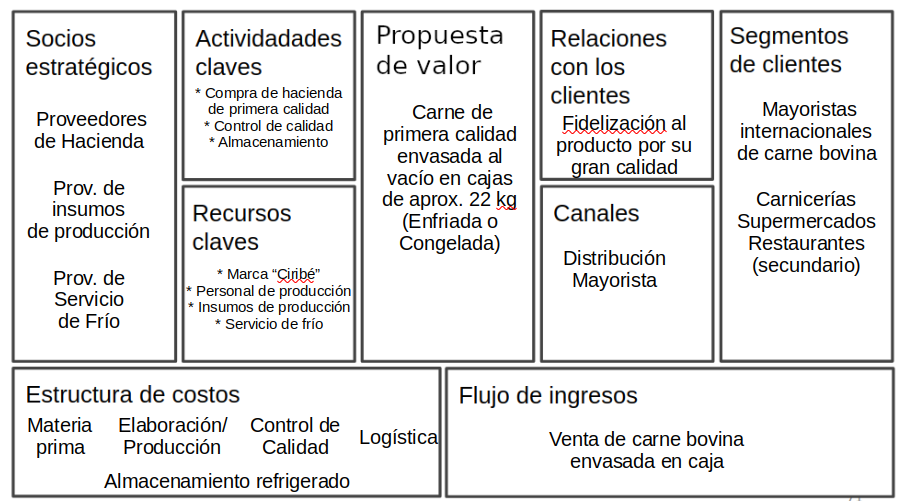
\includegraphics[width=.75\textwidth]{./Figuras/canvasdone.png}
\caption{Modelo Canvas}
\label{fig:canvasdone}
\end{figure}

Comprendiendo la importancia de suministrar alimentos seguros y saludables, la Dirección de la Empresa, toma el compromiso de implementar y mantener un sistema de Control de Calidad basado en los lineamientos del Sistema de Análisis de Riesgos y Puntos Críticos de Control (HACCP), para todos sus productos. Debido a esto, el control de temperatura tanto de carnes como de cámaras de almacenamiento, juega un papel fundamental. Además, al ser una central frigorífica con casi 22 años de edad, es imperioso contar con un sistema de monitoreo en tiempo real de las instalaciones críticas para poder predecir anomalías que pueden ser de un costo muy significativo para la empresa y su misión.

En cuanto a la parte técnica, la central de frío del túnel de congelado consta de dos compresores alemanes marca Bock de 25 hp, un banco de condensadores, dos placas de intercambio y un circuito con una bomba de circulación de agua y glicol que enfría las placas de congelamiento por contacto. Como se puede observar en la figura \ref{fig:circuito_tunel}, la central de refrigeración realiza su ciclo normal de enfriado con el objetivo de llevar el líquido circulante a temperaturas bajo cero, mientras es conducido hacia las estanterías de congelado por contacto.

\begin{figure}[htpb]
\centering 
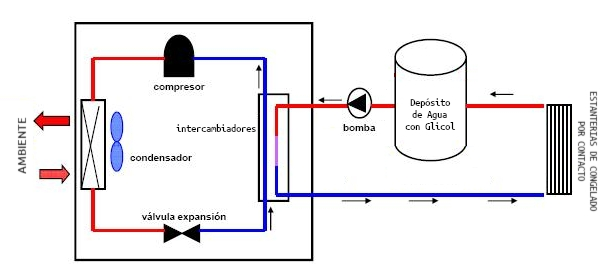
\includegraphics[width=.7\textwidth]{./Figuras/circuito_tunel.png}
\caption{Ciclo de refrigeración con depósito de agua y glicol}
\label{fig:circuito_tunel}
\end{figure}

A nivel general, el sistema debe poder cumplir con el objetivo de predecir fallas y alertar ante situaciones críticas que surjan del monitoreo de la central y, de esta manera, lograr reducir los costos de mantenimiento prolongando el tiempo de uso de los equipos. Para poder cumplir con estos requerimientos se necesitan medir los siguientes puntos:
\begin{itemize}
	\item Consumo en Amperes de cada compresor,
	\item Temperatura de succión y de salida de cada compresor,
	\item Temperatura de los intercambiadores,	
	\item Temperatura de retorno del banco de condensadores,
	\item Consumo en Amperes de la bomba de agua,
	\item Temperatura de cada estantería de congelado por contacto,
	\item Temperatura ambiente del túnel de congelado, y
	\item Temperatura exterior (ambiental).
\end{itemize}

Cada uno de estos puntos de sensado proporciona datos que pueden ser transformados en información extremadamente útil. Por ejemplo, una temperatura de succión muy baja, por un período de tiempo prolongado, puede indicar que está retornando líquido al compresor, lo cual es de una gravedad considerable.

Siguiendo el comportamiento del sistema que ya ha sido implementado parcialmente por la empresa (ver figura \ref{fig:diagramabloques}), la información recolectada por el hardware de monitoreo debe enviarse por WiFi al servidor Blynk a través del protocolo MQTT. El servidor Blynk presenta una API REST para que los datos puedan ser accedidos desde Python y almacenados en una base de datos PostgreSQL para su posterior utilización y análisis. Al momento de ir sensando y recolectando cada dato se ejecutan las validaciones correspondientes que activan alertas por correo electrónico al personal de mantenimiento. A su vez, los usuarios pueden visualizar los datos en tiempo real desde la aplicación en Blynk, ya sea dentro o fuera de la empresa, en cuyo caso la conexión se realiza a través de una red privada virtual (VPN). Para consultar, visualizar o graficar la información recolectada se utilizan páginas web en Django; y en determinados puntos críticos de control se puede acceder a información histórica específica a través de web services.

\begin{figure}[htpb]
\centering 
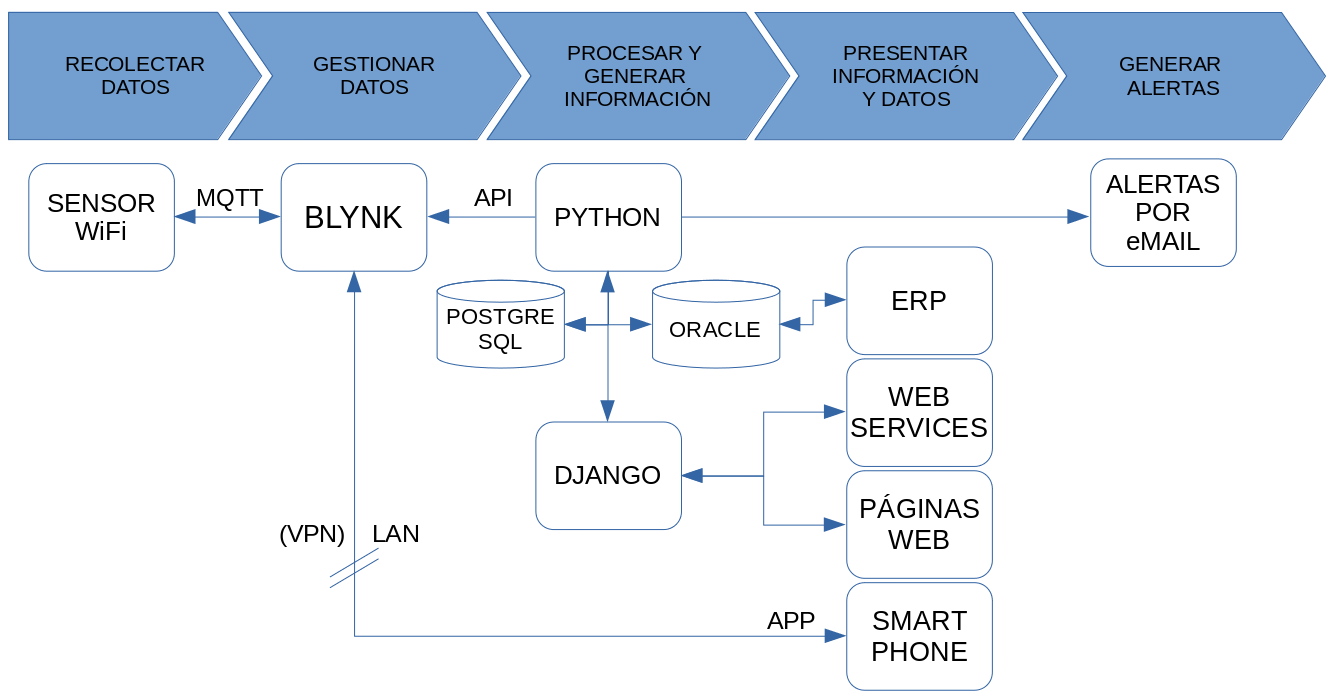
\includegraphics[width=.9\textwidth]{./Figuras/diagramabloques.png}
\caption{Diagrama de bloques del sistema}
\label{fig:diagramabloques}
\end{figure}

\section{Identificación y análisis de los interesados}
\label{sec:interesados}

A continuación se pueden observar las personas interesadas en este proyecto y el rol que cada una va a desempeñar.
\begin{table}[ht]
%\caption{Identificación de los interesados}
%\label{tab:interesados}
\begin{tabularx}{\linewidth}{@{}|l|X|X|l|@{}}
\hline
\rowcolor[HTML]{C0C0C0} 
Rol           & Nombre y Apellido & Organización 	& Puesto 	\\ \hline
Auspiciante   & \clientename      &\empclientename	& Presidente 	\\ \hline
Cliente       & \clientename      &\empclientename	&Presidente 		\\ \hline
Impulsor      & Hernán Ciribé	 &\empclientename	&Gerente Gral.		\\ \hline
Responsable   & \authorname       & FIUBA        	& Alumno 	\\ \hline
Colaboradores & Andrés Giacomino  &YACO Refrigeración 	&Dueño       	\\ \hline
Orientador    & \supname	      & \pertesupname 	& Director Trabajo final \\ \hline
Equipo        & Lucas Tondo \newline 
				Ignacio Abendaño          &\empclientename &Operarios Mantenimiento        	\\ \hline
Usuario final &Lucas Tondo \newline 
				Ignacio Abendaño \newline 
				Hernán Ciribé  \newline 
				Leandro Ciribé &\empclientename	&Gerencia y Mantenimiento \\ \hline
\end{tabularx}
\end{table}

Las principales características de cada interesado son:
\begin{itemize}
	\item Auspiciante: está muy interesado en poder reducir los costos de mantenimiento. Estima realizar una inversión inferior al costo del arreglo de un compresor, que puede llegar a rondar los 40.000 pesos.
	\item Cliente: es una persona que necesita poder constatar las mejoras obtenidas, en cuanto a ahorro monetario, debido a un mantenimiento preventivo realizado correctamente y a tiempo.
	\item Impulsor: persona que está muy interesada en incorporar adelantos tecnológicos que reduzcan los costos y mejoren la operatoria de la empresa.
	\item Responsable: está muy interesado en maximizar el tiempo de disponibilidad de los equipamientos y reducir los índices de roturas particularmente en compresores.
	\item Colaboradores: es la persona indicada para ayudar a evacuar cualquier duda sobre tecnologías de centrales frigoríficas. Tener en cuenta que a veces su tiempo disponible es escaso.
	\item Orientador: es una persona idónea para consultar y definir los objetivos a seguir en el proyecto.
	\item Equipo: ambas personas son responsables y proactivas en incorporar nuevas tecnologías que mejoren su trabajo.
	\item Usuario Final: están urgidos en disponer de la información para poder tomar las mejores decisiones dentro de su área de trabajo.
\end{itemize}

\section{1. Propósito del proyecto}
\label{sec:proposito}

El propósito de este proyecto es disponer de información útil para identificar cambios en el comportamiento normal de una central de frío, poder aprender a predecir fallas que sean de un costo significativo para la empresa y maximizar el tiempo de disponibilidad de la central frigorífica.

\section{2. Alcance del proyecto}
\label{sec:alcance}

En el presente proyecto se incorporarán nuevos sensores para medir el consumo de cada compresor y sensores de temperatura en lugares claves de la central del túnel de congelado (como ya se ha detallado anteriormente en este documento). También se utilizarán datos de sensores ya existentes en el sistema y se incorporarán las líneas de código necesarias para adaptar los nuevos sensores al sistema vigente. En el proyecto no se incluye el sensado de presión, como así tampoco el monitoreo de la central de media temperatura que será implementado en una etapa posterior.

\section{3. Supuestos del proyecto}
\label{sec:supuestos}

Para el desarrollo del presente proyecto se supone que:
\begin{itemize}
	\item La empresa dispondrá de los materiales necesarios, como por ejemplo los controladores WiFi y demás sensores.
	\item El personal de mantenimiento asistirá en las tareas de instalación y conexión del hardware.
	\item El área de informática otorgará los permisos y la infraestructura necesaria para la implementación.
\end{itemize}

\section{4. Requerimientos}
\label{sec:requerimientos}

Se detallan a continuación los distintos requerimientos del sistema.
\begin{enumerate}
	\item Requerimientos técnicos
		\begin{enumerate}
			\item Los valores sensados por el hardware deben transmitirse por WiFi al SSID: IOT\_FRIGOR
			\item La red WiFi debe ser de 2.4Ghz con seguridad WPA/WPA2-Personal y encriptación AES o TKIP
			\item Se debe disponer de línea de UPS en el sector para la conexión segura del hardware de monitoreo
		\end{enumerate}
	\item Requerimientos funcionales
		\begin{enumerate}
			\item El sistema debe medir el consumo en amperes del compresor N°1
			\item El sistema debe medir el consumo en amperes del compresor N°2
			\item El sistema debe medir el consumo en amperes de la bomba recirculadora
			\item El sistema debe medir la temperatura de succión del compresor N°1
			\item El sistema debe medir la temperatura de succión del compresor N°2
			\item El sistema debe medir la temperatura de salida de compresión del compresor N°1
			\item El sistema debe medir la temperatura de salida de compresión del compresor N°2
			\item El sistema debe medir la temperatura de entrada de los intercambiadores
			\item El sistema debe medir la temperatura de salida de los intercambiadores
			\item El sistema debe medir la temperatura de retorno del banco de condensadores
			\item El usuario debe poder visualizar en tiempo real los valores sensados desde su teléfono celular
			\item El sistema debe alertar por correo electrónico cualquier desvío
		\end{enumerate}
	\item Requerimientos de documentación
		\begin{enumerate}		
			\item Se debe realizar un diagrama funcional del sistema legacy
			\item Se debe realizar un diagrama esquemático de las conexiones del hardware de monitoreo a utilizar
			\item Se debe realizar un diagrama de la instalación física a realizar
			\item Se debe realizar un diagrama de flujos del sistema de alertas
		\end{enumerate}
	\item Requerimiento de testing
		\begin{enumerate}		
			\item Se debe realizar una prueba individual de cada sensor en laboratorio
			\item Se debe realizar una prueba parcial del funcionamiento del hardware de monitoreo en laboratorio
			\item Se debe realizar una prueba de las modificaciones realizadas al software principal en laboratorio
			\item Se debe realizar una prueba del sistema de alertas en laboratorio
			\item Se debe realizar una prueba final completa de toda la instalación antes de la puesta en marcha
		\end{enumerate}
	\item Requerimientos de la interfaz
		\begin{enumerate}		
			\item Se debe utilizar la interfaz de la plataforma Blynk
		\end{enumerate}
	\item Requerimientos interoperabilidad
		\begin{enumerate}		
			\item El nuevo módulo de monitoreo del túnel de congelado debe quedar integrado al sistema legacy
		\end{enumerate}
\end{enumerate}

\section{5. Historias de usuarios (\textit{Product backlog})}
\label{sec:backlog}

Como encargado de mantenimiento quiero saber si un compresor presenta algún problema. Ponderación: 5+5+2=12, Story Point: 13

Como encargado de mantenimiento quiero saber si la central no está funcionando como debería. Ponderación: 5+5+2=12, Story Point: 13

Como encargado de mantenimiento quiero tener información que me oriente rápidamente por dónde puede estar el desperfecto. Ponderación: 5+13+5=23, Story Point: 21

Como encargado de mantenimiento quiero enterarme al instante de cualquier falla en la central de congelado. Ponderación: 3+1+2=6, Story Point: 5

Como usuario quiero saber si existe un problema de temperatura en el túnel de congelado. Ponderación: 3+1+2=6, Story Point: 5

Como personal de mantenimiento quiero poder contrastar los valores medidos con los observados. Ponderación: 1+1+2=4, Story Point: 3

Como gerente general quiero saber si un problema en la central de frío se extiende en el tiempo. Ponderación: 5+5+5=15, Story Point: 13


Criterios que se toman para calcular los \textit{story points} de cada historia:

\begin{table}[ht]
%\caption{Criterios para story points}
\begin{tabularx}{\linewidth}{@{}|X|X|X|X|@{}}
\hline
\rowcolor[HTML]{C0C0C0} 
Pesos criterios  & Bajo & Medio	& Alto \\ \hline
A) Dificultad    & 1    & 3      & 5 \\ \hline
B) Complejidad   & 1    & 5      & 13 \\ \hline
C) Incertidumbre & 2	    & 3      & 5	 \\ \hline
\end{tabularx}
\end{table}

\section{6. Entregables principales del proyecto}
\label{sec:entregables}
Los entregables del proyecto son:
\begin{itemize}
	\item Guía rápida de uso
	\item Diagrama de circuitos esquemáticos
	\item Plaqueta del hardware desarrollado
	\item Código fuente del firmware
	\item Diagrama de instalación
	\item Informe final
\end{itemize}

\section{7. Desglose del trabajo en tareas}
\label{sec:wbs}

El proyecto consta de las siguientes tareas:

\begin{enumerate}
\item Gestión del Proyecto (140 hs)
	\begin{enumerate}
	\item Planificación y presentación del trabajo final (40 hs)
	\item Realizar el informe de avance (20 hs)
	\item Realizar la memoria del trabajo (40 hs)
	\item Preparar la presentación final (40 hs)
	\end{enumerate}
\item Diseño e implementación del hardware (195 hs)
	\begin{enumerate}
	\item Selección de hardware de control y especificación de sensores (25 hs)
	\item Estudio de hojas de datos (25 hs)
	\item Diseño de circuito esquemático (25 hs)
	\item Compra de componentes (10 hs)
	\item Elaboración de plaqueta (40 hs)
	\item Soldado de componentes en plaqueta (20 hs)
	\item Verificación de sensores en plaqueta (20 hs)
	\item Prueba integral de la plaqueta (30 hs)
	\end{enumerate}
\item Diseño e implementación del firmware (130 hs)
	\begin{enumerate}
	\item Estudio del framework Blynk (20 hs)
	\item Programación del firmware (40 hs)
	\item Configuración de Blynk (30 hs)
	\item Implementación del firmware y pruebas (40 hs)
	\end{enumerate}
\item Diseño e implementación del software (135 hs)
	\begin{enumerate}
	\item Estudio y revisión del sistema legacy (25 hs)
	\item Análisis de modificaciones a realizar (30 hs)
	\item Programación de modificaciones de software (40 hs)
	\item Implementación del software y pruebas (40 hs)
	\end{enumerate}
\end{enumerate}

Cantidad total de horas: 600 hs
\pagebreak
\section{8. Diagrama de Activity On Node}
\label{sec:AoN}
En la figura \ref{fig:AoN} se puede apreciar el camino crítico del presente proyecto. Las tareas están agrupadas por colores indicando su grupo principal.
\begin{figure}[htpb]
\centering 
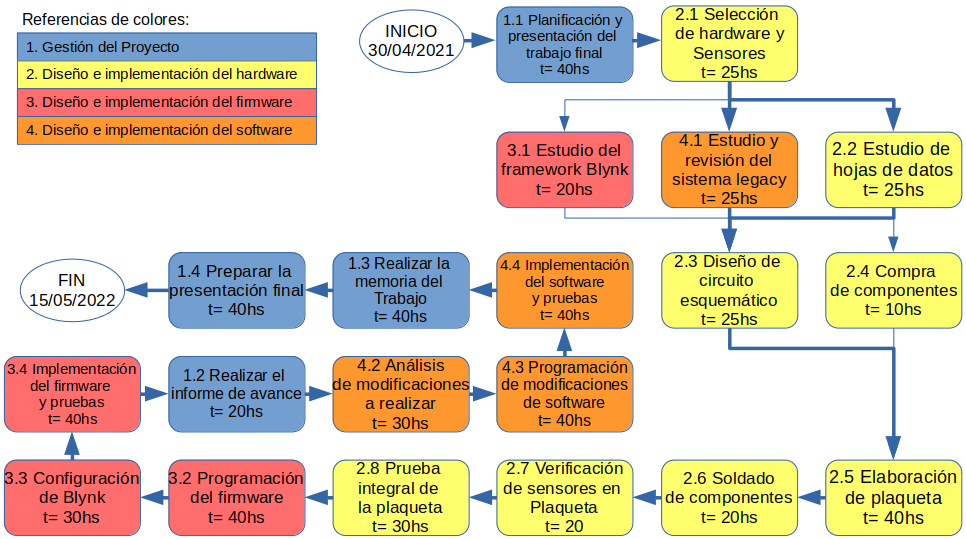
\includegraphics[width=.9\textwidth]{./Figuras/AoN.png}
\caption{Diagrama en \textit{Activity on Node}}
\label{fig:AoN}
\end{figure}

\section{9. Diagrama de Gantt}
\label{sec:gantt}

El siguiente diagrama nos muestra la planificación completa de nuestro proyecto discriminando sus tareas y responsables a lo largo del tiempo.

\begin{figure}[htpb]
\centering 
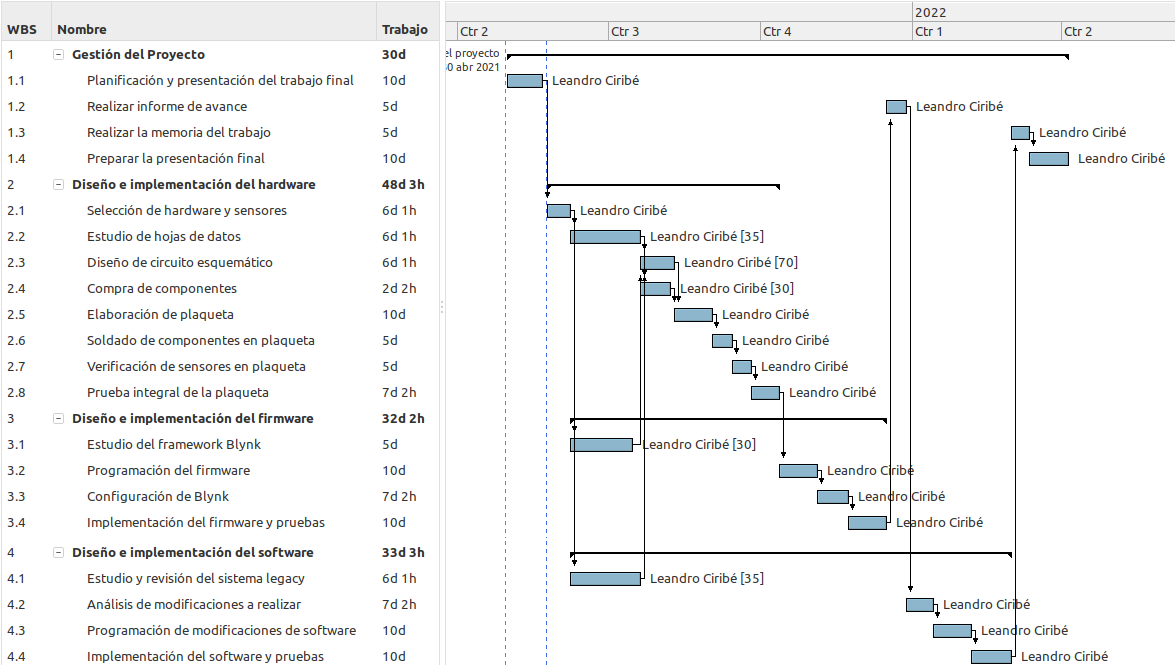
\includegraphics[width=.9\textwidth]{./Figuras/gantt.png}
\caption{\textit{Diagrama de Gantt}}
\label{fig:gantt}
\end{figure}

\section{10. Presupuesto detallado del proyecto}
\label{sec:presupuesto}
Para la elaboración del presupuesto no se incluyó el costo de horas de desarrollo porque se realiza con recursos humanos propios de la empresa. Los costos indirectos fueron estimados como el 29\% de los costos directos, en una primera aproximación.

\begin{table}[htpb]
\centering
\begin{tabularx}{\linewidth}{@{}|X|c|r|r|@{}}
\hline
\rowcolor[HTML]{C0C0C0} 
\multicolumn{4}{|c|}{\cellcolor[HTML]{C0C0C0}COSTOS DIRECTOS} \\ \hline
\rowcolor[HTML]{C0C0C0} 
Descripción &
  \multicolumn{1}{c|}{\cellcolor[HTML]{C0C0C0}Cantidad} &
  \multicolumn{1}{c|}{\cellcolor[HTML]{C0C0C0}Valor unitario} &
  \multicolumn{1}{c|}{\cellcolor[HTML]{C0C0C0}Valor total} \\ \hline
Sensores de Temperatura DS18B20 &
  \multicolumn{1}{c|}{7} &
  \multicolumn{1}{c|}{400} &
  \multicolumn{1}{c|}{2800} \\ \hline
Sensor de Corriente 100A SCT013 &
  \multicolumn{1}{c|}{9} &
  \multicolumn{1}{c|}{1900} &
  \multicolumn{1}{c|}{17100} \\ \hline
NodeMcu ESP32 &
  \multicolumn{1}{c|}{2} &
  \multicolumn{1}{c|}{1500} &
  \multicolumn{1}{c|}{3000} \\ \hline
Plaqueta universal para PCB &
  \multicolumn{1}{c|}{1} &
  \multicolumn{1}{c|}{2000} &
  \multicolumn{1}{c|}{2000} \\ \hline
Otros Insumos y componentes electrónicos &
  \multicolumn{1}{c|}{1} &
  \multicolumn{1}{c|}{3100} &
  \multicolumn{1}{c|}{3100} \\ \hline
Encomiendas, viáticos y gastos varios &
  \multicolumn{1}{c|}{1} &
  \multicolumn{1}{c|}{3000} &
  \multicolumn{1}{c|}{3000} \\ \hline
\multicolumn{3}{|c|}{SUBTOTAL} &
  \multicolumn{1}{c|}{31000} \\ \hline
\rowcolor[HTML]{C0C0C0} 
\multicolumn{4}{|c|}{\cellcolor[HTML]{C0C0C0}COSTOS INDIRECTOS} \\ \hline
\rowcolor[HTML]{C0C0C0} 
Descripción &
  \multicolumn{1}{c|}{\cellcolor[HTML]{C0C0C0}Cantidad} &
  \multicolumn{1}{c|}{\cellcolor[HTML]{C0C0C0}Valor unitario} &
  \multicolumn{1}{c|}{\cellcolor[HTML]{C0C0C0}Valor total} \\ \hline
29 \% de los costos directos&
  \multicolumn{1}{c|}{-} &
  \multicolumn{1}{c|}{-} &
  \multicolumn{1}{c|}{9000} \\ \hline
\multicolumn{3}{|c|}{SUBTOTAL} &
  \multicolumn{1}{c|}{9000} \\ \hline
\rowcolor[HTML]{C0C0C0}
\multicolumn{3}{|c|}{TOTAL} &40000
   \\ \hline
\end{tabularx}%
\end{table}

\section{11. Gestión de riesgos}
\label{sec:riesgos}

Los riesgos que figuran a continuación serán cuantificados de acuerdo a los siguientes parámetros:
\begin{itemize}
	\item Severidad (S): mientras más severo es el riesgo, más alto es el número a utilizar. Rango del 1 al 10.\\
	\item Probabilidad de ocurrencia (O): mientras más probable es que ocurra el riesgo, más alto es el número. Rango del 1 al 10.\\
\end{itemize}   

Riesgo 1: No cumplir con la fecha de entrega acordada.
\begin{itemize}
	\item Severidad (10): este riesgo conlleva a no poder aprobar la especialización en IoT.\\
	\item Ocurrencia (6): dado que el proyecto será realizado en horas de trabajo se podrían estirar los plazos de entrega. Pese a esto, al ser un proyecto importante para la empresa, es posible de que ocurra. \\
\end{itemize}   

Riesgo 2: Cumplir parcialmente con los requerimientos pactados con la empresa.
\begin{itemize}
	\item Severidad (8): conlleva a la entrega de un producto que no funciona como es esperado por el cliente o con funcionalidad disminuida.
	\item Ocurrencia (3): como un sistema similar ya ha sido realizado por la empresa en otros equipos de refrigeración la probabilidad que esto ocurra es muy baja.
\end{itemize}

Riesgo 3: Mala elección del hardware de desarrollo.
\begin{itemize}
	\item Severidad (9): conlleva a la modificación del alcance del proyecto. 
	\item Ocurrencia (8): dado la gran cantidad de sensores a utilizar puede ser que la experiencia previa de la empresa, utilizando hardware más limitado, no sea la adecuada para este proyecto.
\end{itemize}

Riesgo 4: No contar a tiempo con el hardware necesario.
\begin{itemize}
	\item Severidad (10): conlleva a no poder realizar el proyecto.
	\item Ocurrencia (2): algunos sensores ya han sido comprados y otros componentes, que son fáciles de conseguir, están por encargarse.
\end{itemize}

Riesgo 5: Cancelación del proyecto por parte de la empresa.
\begin{itemize}
	\item Severidad (10): conlleva a no poder realizar el proyecto y la no aprobación de la especialización en IoT.
	\item Ocurrencia (1): la ocurrencia es muy baja porque la firma del contrato ya está por realizarse y la empresa está muy interesada en este proyecto.
\end{itemize}


Tabla de gestión de riesgos: (El RPN se calcula como RPN=SxO)

\begin{table}[htpb]
\centering
\begin{tabularx}{\linewidth}{@{}|X|c|c|c|c|c|c|@{}}
\hline
\rowcolor[HTML]{C0C0C0} 
Riesgo & S & O & RPN & S* & O* & RPN* \\ \hline
1-No cumplir con la fecha de entrega acordada       &10   &6   &50 \cellcolor{blue!15}     &9\cellcolor{black!10}    &3\cellcolor{black!10}    &27\cellcolor{blue!35}      \\ \hline
2-Cumplir parcialmente con los requerimientos pactados con la empresa      &8   &3   &24     &    &    &      \\ \hline
3-Mala elección del hardware de desarrollo       &9  &8   &72 \cellcolor{blue!15}     &7\cellcolor{black!10}    &4\cellcolor{black!10}    &28\cellcolor{blue!35}      \\ \hline
4-No contar a tiempo con el hardware necesario       &10   &2   &20     &    &    &      \\ \hline
5-Cancelación del proyecto por parte de la empresa       &10   &1   &10    &    &    &      \\ \hline
\end{tabularx}%
\end{table}

Criterio adoptado:

- Se tomarán medidas de mitigación en los riesgos cuyos números de RPN sean mayores a 35

Nota: los valores marcados con (*) en la tabla corresponden luego de haber aplicado la mitigación. Ambos casos se aprecian resaltados en colores.

Plan de mitigación de los riesgos que originalmente excedían el RPN máximo establecido:
 
Riesgo 1: No cumplir con la fecha de entrega acordada.
\begin{itemize}
	\item Plan de mitigación: poner énfasis en el seguimiento y control del plan de trabajo. Asignar horas no planificadas fuera del horario de trabajo.
	\item Severidad (9): la severidad bajará levemente sabiendo que se trabajará después de hora en caso que sea necesario para mitigar el riesgo. Pero sigue siendo alta si no se cumple la fecha de entrega.
	\item Ocurrencia (3): al poner especial énfasis en la gestión del plan de trabajo y en la posibilidad de uso de horas fuera del horario laboral, la probabilidad de ocurrencia baja a la mitad.
\end{itemize}

Riesgo 3: Mala elección del hardware de desarrollo.
\begin{itemize}
	\item Plan de mitigación: profundo estudio de las distintas placas disponibles en el mercado antes de la elección.
	\item Severidad (7): la severidad bajará sabiendo que se profundizará en el estudio del hardware a utilizar. Pero sigue siendo alto el impacto si se necesita cambiar de placa.
	\item Ocurrencia (4): al estudiar en profundidad cada placa, la probabilidad de esta ocurrencia disminuye notablemente.
\end{itemize}

\section{12. Gestión de la calidad}
\label{sec:calidad}

A continuación se detallan todos los requerimientos del sistema junto con la verificación y validación a ser llevada a cabo por parte del responsable del proyecto.
\begin{enumerate}
	\item Requerimientos técnicos
		\begin{enumerate}
			\item Los valores sensados por el hardware deben transmitirse por WiFi al SSID: IOT\_FRIGOR:
			\begin{itemize}
				\item Verificación: revisar que el firmware apunte en su configuración de WiFi al SSID mencionado.
				\item Validación: probar la comunicación por WiFi y su conexión satisfactoria.
			\end{itemize}
			\item La red WiFi debe ser de 2.4Ghz con seguridad WPA/WPA2-Personal y encriptación AES o TKIP
			\begin{itemize}
				\item Verificación: revisar que el hardware elegido soporte esta frecuencia y niveles de seguridad.
				\item Validación: realizar una conexión del hardware por WiFi y que su conexión sea satisfactoria.
			\end{itemize}
			\item Se debe disponer de línea de UPS en el sector para la conexión segura del hardware de monitoreo
			\begin{itemize}
				\item Verificación: revisar que llegue 220 V de UPS al sector en cuestión.
				\item Validación: realizar la conexión de cualquier dispositivo de 220 V y proceder a cortar la energía eléctrica para validar su correcto funcionamiento.
			\end{itemize}
		\end{enumerate}
	\item Requerimientos funcionales
		\begin{enumerate}
			\item El sistema debe medir el consumo en amperes del compresor N°1
			\begin{itemize}
				\item Verificación: solicitar el consumo del compresor al sector mantenimiento y verificar que la medición sea similar.
				\item Validación: realizar una medición con pinza amperométrica y contrastar valores.
			\end{itemize}
			\item El sistema debe medir el consumo en amperes del compresor N°2
			\begin{itemize}
				\item Verificación: solicitar el consumo del compresor al sector mantenimiento y verificar que la medición sea similar.
				\item Validación: realizar una medición con pinza amperométrica y contrastar valores.
			\end{itemize}
			\item El sistema debe medir el consumo en amperes de la bomba recirculadora
			\begin{itemize}
				\item Verificación: solicitar el consumo de la bomba recirculadora al sector mantenimiento y verificar que la medición sea similar.
				\item Validación: realizar una medición con pinza amperométrica y contrastar valores.
			\end{itemize}
			\item El sistema debe medir la temperatura de succión del compresor N°1
			\begin{itemize}
				\item Verificación: solicitar la gráfica de temperaturas de succión al sector mantenimiento y verificar que la medición sea aproximada.
				\item Validación: realizar una medición con termómetro patrón láser y contrastar valores.
			\end{itemize}
			\item El sistema debe medir la temperatura de succión del compresor N°2
			\begin{itemize}
				\item Verificación: solicitar la gráfica de temperaturas de succión al sector mantenimiento y verificar que la medición sea aproximada.
				\item Validación: realizar una medición con termómetro patrón láser y contrastar valores.
			\end{itemize}
			\item El sistema debe medir la temperatura de salida de compresión del compresor N°1
			\begin{itemize}
				\item Verificación: solicitar la gráfica de temperaturas de salida al sector mantenimiento y verificar que la medición sea aproximada.
				\item Validación: realizar una medición con termómetro patrón láser y contrastar valores.
			\end{itemize}
			\item El sistema debe medir la temperatura de salida de compresión del compresor N°2
			\begin{itemize}
				\item Verificación: solicitar la gráfica de temperaturas de salida al sector mantenimiento y verificar que la medición sea aproximada.
				\item Validación: realizar una medición con termómetro patrón láser y contrastar valores.
			\end{itemize}
			\item El sistema debe medir la temperatura de entrada de los intercambiadores
			\begin{itemize}
				\item Verificación: inspeccionar visualmente la temperatura del intercambiador en el tablero principal y verificar que la medición sea similar.
				\item Validación: realizar una medición con termómetro patrón láser y contrastar valores.
			\end{itemize}
			\item El sistema debe medir la temperatura de salida de los intercambiadores
			\begin{itemize}
				\item Verificación: inspeccionar visualmente la temperatura del intercambiador en el tablero principal y verificar que la medición sea similar.
				\item Validación: realizar una medición con termómetro patrón láser y contrastar valores.
			\end{itemize}
			\item El sistema debe medir la temperatura de retorno del banco de condensadores
			\begin{itemize}
				\item Verificación: solicitar la gráfica de temperaturas de retorno al sector mantenimiento y verificar que la medición sea aproximada.
				\item Validación: realizar una medición con termómetro patrón láser y contrastar valores.
			\end{itemize}
			\item El usuario debe poder visualizar en tiempo real los valores sensados desde su teléfono celular
			\begin{itemize}
				\item Verificación: abrir la aplicación y visualizar valores en tiempo real.
				\item Validación: Contrastar valores visualizados en tiempo real contra tablero principal y medición a través de instrumentos patrones.
			\end{itemize}
			\item El sistema debe alertar por correo electrónico cualquier desvío
			\begin{itemize}
				\item Verificación: ejecutar un script de programación para verificar el correcto envío del correo electrónico.
				\item Validación: realizar casos de prueba donde se superen los umbrales de notificación y validar la llegada del correo electrónico correspondiente.
			\end{itemize}
		\end{enumerate}
	\item Requerimientos de documentación
		\begin{enumerate}		
			\item Se debe realizar un diagrama funcional del sistema legacy
			\begin{itemize}
				\item Verificación: comprobar que el diagrama sea acorde al funcionamiento del sistema legacy.
				\item Validación: realizar varios casos de prueba del funcionamiento siguiendo el diagrama.
			\end{itemize}
			\item Se debe realizar un diagrama esquemático de las conexiones del hardware de monitoreo a utilizar
			\begin{itemize}
				\item Verificación: comprobar que el diagrama de conexiones sea acorde al hardware realizado.
				\item Validación: realizar pruebas exhaustivas del funcionamiento del hardware.
			\end{itemize}
			\item Se debe realizar un diagrama de la instalación física a realizar
			\begin{itemize}
				\item Verificación: comprobar que el diagrama de instalación sea factible físicamente.
				\item Validación: realizar pruebas de la instalación a realizar.
			\end{itemize}
			\item Se debe realizar un diagrama de flujos del sistema de alertas
			\begin{itemize}
				\item Verificación: comprobar que el diagrama de flujos sea acorde al funcionamiento del sistema de alertas.
				\item Validación: realizar casos de pruebas exhaustivos del funcionamiento de las alertas.
			\end{itemize}
		\end{enumerate}
	\item Requerimiento de testing
		\begin{enumerate}		
			\item Se debe realizar una prueba individual de cada sensor en laboratorio
			\begin{itemize}
				\item Verificación: comprobar el funcionamiento correcto de cada sensor de forma individual y que la medición sea acorde.
				\item Validación: realizar pruebas en distintos valores de medición y contrastar con mediciones de dispositivo patrón.
			\end{itemize}
			\item Se debe realizar una prueba parcial del funcionamiento del hardware de monitoreo en laboratorio
			\begin{itemize}
				\item Verificación: comprobar el funcionamiento correcto del hardware y que los valores obtenidos sean correctos.
				\item Validación: realizar pruebas prolongadas variando los valores sensados y contrastar con mediciones de dispositivo patrón.
			\end{itemize}
			\item Se debe realizar una prueba de las modificaciones realizadas al software principal en laboratorio
			\begin{itemize}
				\item Verificación: comprobar el funcionamiento correcto del software y que las modificaciones realizadas no afecten el funcionamiento general del sistema.
				\item Validación: realizar pruebas exhaustivas del software para validar su funcionamiento.
			\end{itemize}
			\item Se debe realizar una prueba del sistema de alertas en laboratorio
			\begin{itemize}
				\item Verificación: alterar un script de programación para verificar el correcto envío del correo electrónico de alerta.
				\item Validación: tomar un sensor y generarle una variación para que supere los umbrales de notificación y validar la llegada del correo electrónico.
			\end{itemize}
			\item Se debe realizar una prueba final completa de toda la instalación antes de la puesta en marcha
			\begin{itemize}
				\item Verificación: controlar que todos los sensores estén en su lugar y generando sus lecturas.
				\item Validación: poner en marcha el sistema completo y validar con pruebas exhaustivas y prolongadas las funcionalidades requeridas.
			\end{itemize}
		\end{enumerate}
	\item Requerimientos de la interfaz
		\begin{enumerate}		
			\item Se debe utilizar la interfaz de la plataforma Blynk
			\begin{itemize}
				\item Verificación: controlar que todos los valores medidos se puedan visualizar desde la interfase de Blynk.
				\item Validación: mostrar como se visualizan fácilmente los datos medidos en tiempo real y contrastar con sistemas patrones.
			\end{itemize}
		\end{enumerate}
	\item Requerimientos interoperabilidad
		\begin{enumerate}		
			\item El nuevo módulo de monitoreo del túnel de congelado debe quedar integrado al sistema legacy
			\begin{itemize}
				\item Verificación: revisar el nuevo módulo de monitoreo esté integrado al sistema legacy.
				\item Validación: mostrar al cliente que la información necesaria para el sistema legacy es accesible.
			\end{itemize}
		\end{enumerate}
\end{enumerate}

\section{13. Procesos de cierre}    
\label{sec:cierre}

Una vez concluido el proyecto, se procederá a su cierre o proceso de finalización. Para esto, se contemplan las siguientes actividades:
\begin{itemize}
	\item Análisis de las pautas de trabajo:
	\begin{itemize}
		\item Persona responsable: Lic. Leandro Ciribé
		\item Procedimiento: Se analizará si se respetó el plan de proyecto original, contemplando que se haya cumplido con la fecha de finalización pautada, la cantidad de horas asignadas al proyecto y el porcentaje de requerimientos cumplidos.
	 \end{itemize}
	\item Identificación de las técnicas y procedimientos útiles e inútiles que se emplearon, y los problemas que surgieron y cómo se solucionaron:
	\begin{itemize}
		\item Persona responsable: Lic. Leandro Ciribé
		\item Procedimiento: Se analizarán y evaluarán las técnicas y procedimientos que resultaron útiles para lograr los objetivos, su nivel de cumplimiento y las acciones no planificadas que se tomaron para asegurarlos.
	 \end{itemize}
	\item Acto formal de cierre:
	\begin{itemize}
		\item Persona responsable: Lic. Leandro Ciribé
		\item Procedimiento: El responsable del proyecto estará a cargo de realizar el acto de cierre, con el objetivo de agradecer a todos los involucrados en el proyecto, miembros del jurado, docentes y autoridades competentes.
	 \end{itemize}
\end{itemize}

\end{document}
